\chapter{Estado del arte}\label{chap:estado-arte}

En el capítulo anterior se justificó por qué construir un sistema de aprendizaje
federado obliga a apoyarse en \textit{frameworks} especializados. Este capítulo revisa el
panorama de herramientas disponibles, explica con qué criterios se han seleccionado las
tres que se comparan en el trabajo y por qué se han descartado otras, describe cada una
con cierto detalle, las contrasta en una tabla comparativa y, por último, sitúa la
aportación del proyecto frente a los estudios comparativos ya publicados.

\section{Panorama de herramientas existentes}\label{sec:panorama-frameworks}

El número de \textit{frameworks} de aprendizaje federado ha crecido con rapidez en los
últimos años, con propuestas tanto académicas como industriales que responden a
prioridades muy distintas \parencite{riedel2024comparative}. Esa diversidad complica la
elección, porque dos herramientas pueden resolver el mismo problema con arquitecturas,
APIs y modos de ejecución muy diferentes \parencite{bonawitz2019towards}. A grandes
rasgos, las herramientas más conocidas pueden agruparse según su orientación dominante.

Un primer grupo está formado por herramientas orientadas a la investigación y la
experimentación. TensorFlow Federated, desarrollado por Google sobre TensorFlow, expone
la lógica federada mediante una API funcional y un entorno de simulación pensado para
prototipar algoritmos \parencite{tff2019}. FedML se presenta como biblioteca de
investigación y banco de pruebas, con implementaciones de referencia que facilitan
comparaciones reproducibles \parencite{he2020fedml}. Flower, por su parte, prioriza la
facilidad de uso y la independencia respecto de la biblioteca de aprendizaje, lo que lo
ha popularizado en entornos académicos \parencite{beutel2020flower}.

Un segundo grupo se orienta hacia la privacidad y los entornos de producción. PySyft, de
la comunidad OpenMined, se centra en técnicas de protección de datos como la privacidad
diferencial y el cómputo seguro multiparte \parencite{ryffel2018generic}. FATE, de
WeBank, está orientado a aplicaciones industriales y ofrece soporte para aprendizaje
horizontal, vertical y por transferencia con fuertes garantías de protección de datos
\parencite{liu2021fate}. OpenFL, de Intel, se enfoca a escenarios \textit{cross-silo} y
ha tenido especial aceptación en el ámbito sanitario \parencite{reina2021openfl}. NVIDIA
FLARE se sitúa también en esta franja, con énfasis en el paso de la simulación al
despliegue real y en la seguridad integrada \parencite{roth2022nvflare}.

Como cada herramienta responde a un conjunto de prioridades, no existe un único
\textit{framework} de referencia válido para todos los casos. Un trabajo reciente comparó
quince herramientas de código abierto mediante un esquema de puntuación ponderado y situó
a Flower en primera posición por características, interoperabilidad y facilidad de uso, por
delante de FedML, FATE o TensorFlow Federated \parencite{riedel2024comparative}. Sobre
este panorama, el presente trabajo selecciona tres herramientas con enfoques
complementarios: Flower, NVIDIA FLARE y FedML.

\section{Criterios de selección}\label{sec:criterios-seleccion}

La selección de los \textit{frameworks} comparados responde a varios criterios. Se ha
buscado, en primer lugar, que las herramientas estén en mantenimiento activo, con
versiones recientes y documentación al día, para que la comparación tenga validez en el
momento de realizarse. En segundo lugar, se ha valorado que sean agnósticas respecto de
la biblioteca de aprendizaje, de modo que el mismo modelo en PyTorch pueda ejecutarse en
todas y la comparación no quede contaminada por diferencias de implementación del modelo.
En tercer lugar, se ha exigido que ofrezcan un modo de simulación capaz de ejecutarse en
una única máquina con una sola GPU, dado el entorno experimental disponible. Por último,
se ha procurado que los tres representen filosofías de diseño distintas, de manera que la
comparación resulte informativa.

Con esos criterios, varias herramientas conocidas quedan fuera del estudio. TensorFlow
Federated se ha descartado porque su actividad de desarrollo se ha reducido de forma
notable y no publica versiones nuevas desde hace tiempo, lo que lo hace poco recomendable
para un trabajo que pretende comparar herramientas vigentes \parencite{tff2019}; a ello se
añade que su API funcional y su fuerte acoplamiento a TensorFlow encajan mal con un
experimento basado en PyTorch. FATE, pese a su madurez industrial, está concebido para
despliegues empresariales de gran escala y su instalación y configuración resultan
considerablemente más pesadas de lo que requiere un estudio comparativo controlado, con
un enfoque orientado sobre todo al aprendizaje vertical entre organizaciones
\parencite{liu2021fate}. OpenFL se ha descartado por su orientación más estrecha a
escenarios \textit{cross-silo} concretos y por una comunidad y un ecosistema de ejemplos
menores que los de las alternativas elegidas \parencite{reina2021openfl}. PySyft, por
último, sitúa el acento en la privacidad y en el cómputo seguro más que en la comparación
de rendimiento, y su abstracción difiere lo suficiente como para dificultar una
comparación homogénea con las demás \parencite{ryffel2018generic}.

Frente a estas, las tres herramientas seleccionadas cumplen los criterios y cubren
prioridades complementarias: Flower aporta la perspectiva de investigación centrada en la
facilidad de uso, NVIDIA FLARE la de la transición hacia producción con seguridad
integrada y FedML la del banco de pruebas reproducible. Que las tres sean agnósticas
respecto de la biblioteca de aprendizaje y dispongan de un modo de simulación en una sola
máquina permite ejecutar en todas un mismo experimento en PyTorch bajo condiciones
equivalentes.

\section{Frameworks seleccionados}\label{sec:frameworks-seleccionados}

Pese a sus distintas orientaciones, los tres \textit{frameworks} comparten una
arquitectura conceptual común, que la Figura~\ref{fig:arquitectura-frameworks} resume en
forma de capas. Sobre el \textit{hardware} de cómputo se apoya un \textit{backend} de
aprendizaje (en este trabajo, PyTorch), encargado de definir y entrenar el modelo. Por
encima, un motor de ejecución y simulación gestiona la creación de los clientes y su
ejecución, ya sea en procesos reales o simulados en una misma máquina. Una capa de
comunicación traslada los modelos entre el servidor y los clientes mediante mecanismos
como gRPC o el paso de mensajes. La estrategia de agregación, situada en el servidor,
decide cómo se combinan los modelos locales (con \textit{FedAvg} como opción habitual). En
la cima, la lógica del experimento define el modelo, el reparto de los datos y las
métricas. Las diferencias entre herramientas no están tanto en la existencia de estas
capas como en cómo las exponen al desarrollador y en qué énfasis ponen en cada una.

\begin{figure}[htbp]
  \centering
  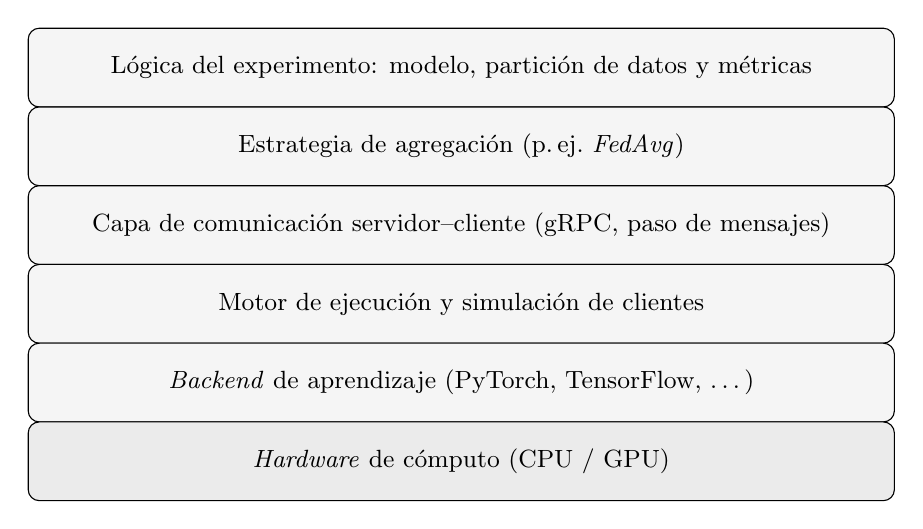
\begin{tikzpicture}[
      every node/.style={font=\small, align=center},
      capa/.style={draw, rounded corners, minimum width=11cm, minimum height=1cm, inner sep=4pt, fill=gray!8}
    ]
    \node[capa] (app)   at (0,5)  {Lógica del experimento: modelo, partición de datos y métricas};
    \node[capa] (strat) at (0,4)  {Estrategia de agregación (p.\,ej.\ \textit{FedAvg})};
    \node[capa] (comm)  at (0,3)  {Capa de comunicación servidor--cliente (gRPC, paso de mensajes)};
    \node[capa] (sim)   at (0,2)  {Motor de ejecución y simulación de clientes};
    \node[capa] (ml)    at (0,1)  {\textit{Backend} de aprendizaje (PyTorch, TensorFlow, \dots)};
    \node[capa, fill=gray!16] (hw) at (0,0) {\textit{Hardware} de cómputo (CPU / GPU)};
  \end{tikzpicture}
  \caption{Arquitectura por capas común a los \textit{frameworks} de aprendizaje
  federado comparados. Las herramientas se diferencian en cómo exponen cada capa al
  desarrollador y en el énfasis que ponen en la simulación, el despliegue o la seguridad.
  Elaboración propia.}
  \label{fig:arquitectura-frameworks}
\end{figure}

\subsection{Flower}\label{sec:ea-flower}

Flower es un \textit{framework} de aprendizaje federado presentado por
\textcite{beutel2020flower} y surgido de un proyecto de investigación universitario. Su
diseño es agnóstico respecto de la biblioteca de aprendizaje automático: el mismo sistema
funciona con PyTorch, TensorFlow u otras, y separa con claridad la lógica del cliente
(\textit{ClientApp}) de la del servidor (\textit{ServerApp}), de modo que el desarrollador
solo implementa las funciones de entrenamiento y evaluación y delega en el
\textit{framework} la coordinación de las rondas \parencite{beutel2020flower}. Está
pensado para experimentos a gran escala y para simular escenarios heterogéneos con muchos
clientes; su motor de simulación permite instanciar numerosos clientes virtuales sobre los
recursos disponibles, lo que lo ha popularizado en investigación. La estrategia de
agregación se configura de forma explícita en el servidor, con \textit{FedAvg} como opción
por defecto y la posibilidad de sustituirla por otras. En el estudio de
\textcite{riedel2024comparative} obtuvo la puntuación más alta entre los quince
\textit{frameworks} analizados, en buena medida por su facilidad de uso y su
interoperabilidad.

\subsection{NVIDIA FLARE}\label{sec:ea-nvflare}

NVIDIA FLARE (\textit{NVIDIA Federated Learning Application Runtime Environment}) es un
SDK de aprendizaje federado desarrollado por NVIDIA y descrito por
\textcite{roth2022nvflare}. Su lema, «de la simulación al mundo real», resume su
orientación: facilitar que un mismo experimento pase de ejecutarse en simulación a
desplegarse en una infraestructura real con cambios mínimos. Es igualmente agnóstico
respecto de la biblioteca de entrenamiento, pues admite PyTorch, TensorFlow, XGBoost o
incluso NumPy, y organiza la ejecución en torno a controladores y \textit{workflows} que
definen cómo se coordinan servidor y clientes \parencite{roth2022nvflare}. Su rasgo más
distintivo es que incorpora de serie mecanismos de seguridad y privacidad, como la
agregación con cifrado homomórfico, la privacidad diferencial o el filtrado de mensajes, y
un modelo de gestión por sitios pensado para entornos con varias organizaciones. Esta
orientación lo acerca a entornos empresariales y de producción, con presencia destacada en
el ámbito sanitario, a costa de una configuración algo más estructurada que la de
herramientas centradas solo en la simulación.

\subsection{FedML}\label{sec:ea-fedml}

FedML es una biblioteca de investigación y banco de pruebas para aprendizaje federado
presentada por \textcite{he2020fedml} y mantenida posteriormente bajo el proyecto
TensorOpera. Su objetivo es facilitar el desarrollo de nuevos algoritmos y permitir
comparaciones justas y reproducibles; para ello ofrece una API flexible e implementaciones
de referencia de optimizadores, modelos y conjuntos de datos, así como una separación
clara entre el entrenador del cliente (\textit{ClientTrainer}) y el agregador del servidor
(\textit{ServerAggregator}) \parencite{he2020fedml}. Admite tres paradigmas de cómputo:
entrenamiento en el dispositivo (\textit{edge}), cómputo distribuido y simulación en una
sola máquina, de modo que un mismo experimento puede ejecutarse en configuraciones
distintas \parencite{he2020fedml}. En su modo de simulación ofrece, además, dos motores de
ejecución (uno secuencial de proceso único y otro basado en paso de mensajes que permite
ejecutar clientes en paralelo), lo que resulta especialmente relevante para estudiar el
comportamiento del \textit{framework} bajo distintas configuraciones de concurrencia.

\section{Comparativa de los frameworks seleccionados}\label{sec:ea-comparativa-frameworks}

La Tabla~\ref{tab:comparativa-frameworks} resume las principales diferencias entre los
tres \textit{frameworks} a partir de la documentación oficial y de la bibliografía
revisada. La comparación se organiza en torno a los aspectos que más influyen en la
elección de una herramienta para un estudio como este: su orientación principal, el
soporte de bibliotecas de aprendizaje, las capacidades de simulación y de despliegue real,
los mecanismos de seguridad integrados, el estado de la documentación, la facilidad de uso
percibida y su adecuación al experimento planteado. Conviene leerla como una síntesis
cualitativa orientativa; las diferencias cuantitativas de rendimiento y consumo se abordan
en los capítulos de resultados.

\begin{table}[htbp]
  \centering
  \caption{Comparación cualitativa de los tres \textit{frameworks} seleccionados.}
  \label{tab:comparativa-frameworks}
  \footnotesize
  \begin{tabular}{p{2.6cm} p{3.2cm} p{3.2cm} p{3.2cm}}
    \toprule
    Aspecto & Flower & NVIDIA FLARE & FedML \\
    \midrule
    Orientación principal & Investigación y prototipado & De la simulación a producción &
    Investigación y \textit{benchmarking} \\
    Soporte de bibliotecas & Agnóstico (PyTorch, TensorFlow, etc.) &
    Agnóstico (PyTorch, TensorFlow, XGBoost, NumPy) & Agnóstico, centrado en PyTorch \\
    Simulación & Motor de simulación a gran escala con clientes virtuales &
    Simulador integrado con paso a despliegue real & Simulación con motor secuencial y
    motor concurrente \\
    Despliegue real & Soportado mediante despliegue de cliente y servidor &
    Eje central del diseño, con gestión por sitios & Soportado, con orientación a
    investigación \\
    Seguridad y privacidad & A cargo del desarrollador o mediante extensiones &
    Integrada (cifrado homomórfico, privacidad diferencial, filtros) &
    Disponible según el paradigma de cómputo \\
    Documentación & Extensa y orientada a ejemplos & Amplia, con enfoque empresarial &
    Amplia pero más fragmentada \\
    Facilidad de uso & Alta, con API sencilla & Media, configuración más estructurada &
    Media, API flexible pero más densa \\
    Adecuación al experimento & Alta: simulación directa en una GPU &
    Alta: simulación controlada y registros detallados & Alta: permite comparar
    configuraciones de concurrencia \\
    \bottomrule
  \end{tabular}
\end{table}

\section{Estudios comparativos previos}\label{sec:comparativas-previas}

Comparar \textit{frameworks} de aprendizaje federado no es una idea nueva, pero la mayoría
de los trabajos publicados se centra en aspectos cualitativos o documentales. El estudio
de \textcite{riedel2024comparative}, ya citado, evalúa quince herramientas según
características, interoperabilidad y facilidad de uso mediante un esquema de puntuación
ponderado, pero no mide cómo se comportan al ejecutar un mismo entrenamiento ni qué
recursos consumen al hacerlo. Otra línea de trabajo analiza el efecto de la heterogeneidad
de los datos sobre la precisión del modelo y muestra cómo las distribuciones no~IID
degradan la convergencia \parencite{li2020federated}, pero lo hace desde una perspectiva
algorítmica, sin atender al coste de ejecución de cada herramienta. Por su parte, los
trabajos que describen cada \textit{framework} suelen proceder de sus propios autores y
presentar las capacidades de la herramienta más que una comparación independiente entre
varias \parencite{beutel2020flower,roth2022nvflare,he2020fedml}.

Queda así un hueco apreciable. Faltan comparaciones experimentales que, partiendo de un
mismo escenario y en condiciones equivalentes, midan a la vez la precisión del modelo y el
consumo de recursos de cada \textit{framework}: tiempo de ejecución, memoria, uso de GPU y
energía estimada, junto con aspectos prácticos como la reproducibilidad o la facilidad de
uso. Cubrir parte de ese hueco es el objetivo de este trabajo.

\section{Síntesis y posicionamiento}\label{sec:sintesis-posicionamiento}

Los tres \textit{frameworks} elegidos cubren prioridades complementarias: Flower apuesta
por la facilidad de uso y la investigación, NVIDIA FLARE por la transición hacia
producción con seguridad integrada y FedML por la reproducibilidad y la comparación de
algoritmos. Comparten, además, una arquitectura conceptual común y la capacidad de
ejecutar en simulación un mismo experimento en PyTorch, lo que los hace idóneos para un
estudio controlado. Ejecutarlos sobre un mismo escenario permite observar cómo esas
decisiones de diseño se traducen en diferencias concretas de rendimiento, consumo de
recursos y experiencia de uso, que es justamente la aportación que persigue este trabajo
frente a los estudios previos. El siguiente capítulo describe la metodología experimental
de esa comparación: el escenario común, el control de variables y las métricas empleadas.
